% Options for packages loaded elsewhere
\PassOptionsToPackage{unicode}{hyperref}
\PassOptionsToPackage{hyphens}{url}
%
\documentclass[
]{report}
\usepackage{amsmath,amssymb}
\usepackage{iftex}
\ifPDFTeX
  \usepackage[T1]{fontenc}
  \usepackage[utf8]{inputenc}
  \usepackage{textcomp} % provide euro and other symbols
\else % if luatex or xetex
  \usepackage{unicode-math} % this also loads fontspec
  \defaultfontfeatures{Scale=MatchLowercase}
  \defaultfontfeatures[\rmfamily]{Ligatures=TeX,Scale=1}
\fi
\usepackage{lmodern}
\ifPDFTeX\else
  % xetex/luatex font selection
\fi
% Use upquote if available, for straight quotes in verbatim environments
\IfFileExists{upquote.sty}{\usepackage{upquote}}{}
\IfFileExists{microtype.sty}{% use microtype if available
  \usepackage[]{microtype}
  \UseMicrotypeSet[protrusion]{basicmath} % disable protrusion for tt fonts
}{}
\makeatletter
\@ifundefined{KOMAClassName}{% if non-KOMA class
  \IfFileExists{parskip.sty}{%
    \usepackage{parskip}
  }{% else
    \setlength{\parindent}{0pt}
    \setlength{\parskip}{6pt plus 2pt minus 1pt}}
}{% if KOMA class
  \KOMAoptions{parskip=half}}
\makeatother
\usepackage{xcolor}
\usepackage{color}
\usepackage{fancyvrb}
\newcommand{\VerbBar}{|}
\newcommand{\VERB}{\Verb[commandchars=\\\{\}]}
\DefineVerbatimEnvironment{Highlighting}{Verbatim}{commandchars=\\\{\}}
% Add ',fontsize=\small' for more characters per line
\usepackage{framed}
\definecolor{shadecolor}{RGB}{248,248,248}
\newenvironment{Shaded}{\begin{snugshade}}{\end{snugshade}}
\newcommand{\AlertTok}[1]{\textcolor[rgb]{0.94,0.16,0.16}{#1}}
\newcommand{\AnnotationTok}[1]{\textcolor[rgb]{0.56,0.35,0.01}{\textbf{\textit{#1}}}}
\newcommand{\AttributeTok}[1]{\textcolor[rgb]{0.13,0.29,0.53}{#1}}
\newcommand{\BaseNTok}[1]{\textcolor[rgb]{0.00,0.00,0.81}{#1}}
\newcommand{\BuiltInTok}[1]{#1}
\newcommand{\CharTok}[1]{\textcolor[rgb]{0.31,0.60,0.02}{#1}}
\newcommand{\CommentTok}[1]{\textcolor[rgb]{0.56,0.35,0.01}{\textit{#1}}}
\newcommand{\CommentVarTok}[1]{\textcolor[rgb]{0.56,0.35,0.01}{\textbf{\textit{#1}}}}
\newcommand{\ConstantTok}[1]{\textcolor[rgb]{0.56,0.35,0.01}{#1}}
\newcommand{\ControlFlowTok}[1]{\textcolor[rgb]{0.13,0.29,0.53}{\textbf{#1}}}
\newcommand{\DataTypeTok}[1]{\textcolor[rgb]{0.13,0.29,0.53}{#1}}
\newcommand{\DecValTok}[1]{\textcolor[rgb]{0.00,0.00,0.81}{#1}}
\newcommand{\DocumentationTok}[1]{\textcolor[rgb]{0.56,0.35,0.01}{\textbf{\textit{#1}}}}
\newcommand{\ErrorTok}[1]{\textcolor[rgb]{0.64,0.00,0.00}{\textbf{#1}}}
\newcommand{\ExtensionTok}[1]{#1}
\newcommand{\FloatTok}[1]{\textcolor[rgb]{0.00,0.00,0.81}{#1}}
\newcommand{\FunctionTok}[1]{\textcolor[rgb]{0.13,0.29,0.53}{\textbf{#1}}}
\newcommand{\ImportTok}[1]{#1}
\newcommand{\InformationTok}[1]{\textcolor[rgb]{0.56,0.35,0.01}{\textbf{\textit{#1}}}}
\newcommand{\KeywordTok}[1]{\textcolor[rgb]{0.13,0.29,0.53}{\textbf{#1}}}
\newcommand{\NormalTok}[1]{#1}
\newcommand{\OperatorTok}[1]{\textcolor[rgb]{0.81,0.36,0.00}{\textbf{#1}}}
\newcommand{\OtherTok}[1]{\textcolor[rgb]{0.56,0.35,0.01}{#1}}
\newcommand{\PreprocessorTok}[1]{\textcolor[rgb]{0.56,0.35,0.01}{\textit{#1}}}
\newcommand{\RegionMarkerTok}[1]{#1}
\newcommand{\SpecialCharTok}[1]{\textcolor[rgb]{0.81,0.36,0.00}{\textbf{#1}}}
\newcommand{\SpecialStringTok}[1]{\textcolor[rgb]{0.31,0.60,0.02}{#1}}
\newcommand{\StringTok}[1]{\textcolor[rgb]{0.31,0.60,0.02}{#1}}
\newcommand{\VariableTok}[1]{\textcolor[rgb]{0.00,0.00,0.00}{#1}}
\newcommand{\VerbatimStringTok}[1]{\textcolor[rgb]{0.31,0.60,0.02}{#1}}
\newcommand{\WarningTok}[1]{\textcolor[rgb]{0.56,0.35,0.01}{\textbf{\textit{#1}}}}
\usepackage{longtable,booktabs,array}
\usepackage{calc} % for calculating minipage widths
% Correct order of tables after \paragraph or \subparagraph
\usepackage{etoolbox}
\makeatletter
\patchcmd\longtable{\par}{\if@noskipsec\mbox{}\fi\par}{}{}
\makeatother
% Allow footnotes in longtable head/foot
\IfFileExists{footnotehyper.sty}{\usepackage{footnotehyper}}{\usepackage{footnote}}
\makesavenoteenv{longtable}
\usepackage{graphicx}
\makeatletter
\def\maxwidth{\ifdim\Gin@nat@width>\linewidth\linewidth\else\Gin@nat@width\fi}
\def\maxheight{\ifdim\Gin@nat@height>\textheight\textheight\else\Gin@nat@height\fi}
\makeatother
% Scale images if necessary, so that they will not overflow the page
% margins by default, and it is still possible to overwrite the defaults
% using explicit options in \includegraphics[width, height, ...]{}
\setkeys{Gin}{width=\maxwidth,height=\maxheight,keepaspectratio}
% Set default figure placement to htbp
\makeatletter
\def\fps@figure{htbp}
\makeatother
\setlength{\emergencystretch}{3em} % prevent overfull lines
\providecommand{\tightlist}{%
  \setlength{\itemsep}{0pt}\setlength{\parskip}{0pt}}
\setcounter{secnumdepth}{5}
% definitions for citeproc citations
\NewDocumentCommand\citeproctext{}{}
\NewDocumentCommand\citeproc{mm}{%
  \begingroup\def\citeproctext{#2}\cite{#1}\endgroup}
\makeatletter
 % allow citations to break across lines
 \let\@cite@ofmt\@firstofone
 % avoid brackets around text for \cite:
 \def\@biblabel#1{}
 \def\@cite#1#2{{#1\if@tempswa , #2\fi}}
\makeatother
\newlength{\cslhangindent}
\setlength{\cslhangindent}{1.5em}
\newlength{\csllabelwidth}
\setlength{\csllabelwidth}{3em}
\newenvironment{CSLReferences}[2] % #1 hanging-indent, #2 entry-spacing
 {\begin{list}{}{%
  \setlength{\itemindent}{0pt}
  \setlength{\leftmargin}{0pt}
  \setlength{\parsep}{0pt}
  % turn on hanging indent if param 1 is 1
  \ifodd #1
   \setlength{\leftmargin}{\cslhangindent}
   \setlength{\itemindent}{-1\cslhangindent}
  \fi
  % set entry spacing
  \setlength{\itemsep}{#2\baselineskip}}}
 {\end{list}}
\usepackage{calc}
\newcommand{\CSLBlock}[1]{\hfill\break\parbox[t]{\linewidth}{\strut\ignorespaces#1\strut}}
\newcommand{\CSLLeftMargin}[1]{\parbox[t]{\csllabelwidth}{\strut#1\strut}}
\newcommand{\CSLRightInline}[1]{\parbox[t]{\linewidth - \csllabelwidth}{\strut#1\strut}}
\newcommand{\CSLIndent}[1]{\hspace{\cslhangindent}#1}
\usepackage{booktabs}
\usepackage{geometry}
\usepackage[none]{hyphenat}
\usepackage{titlesec}
\usepackage{longtable}
\usepackage{xcolor}
\usepackage{setspace}
\usepackage{pdfpages}

\pagestyle{plain}

%%%% Set margins
\setlength{\topmargin}{-1cm}
\addtolength{\evensidemargin}{-1cm}
\addtolength{\oddsidemargin}{-1cm}
\addtolength{\textheight}{3cm}
\addtolength{\textwidth}{2cm}

% Spacing for reading guides
\newcommand{\rgs}{\vspace{12pt}} % Vertical space
\newcommand{\rgi}{\hspace{24pt}}  % Indent

\newcommand\latexcode[1]{#1}

% Format chapter titles and spacing
\renewcommand*{\chaptername}{Module}

\titleformat{\chapter}[display]
{\bfseries\Large}
{\filleft\MakeUppercase{\chaptertitlename} \Huge\thechapter}
{3ex}
{\titlerule
\vspace{1.5ex}%
\filright}
[\vspace{1.5ex}%
\titlerule]
\titlespacing*{\chapter}{0pt}{-40pt}{20pt}
\ifLuaTeX
  \usepackage{selnolig}  % disable illegal ligatures
\fi
\usepackage{bookmark}
\IfFileExists{xurl.sty}{\usepackage{xurl}}{} % add URL line breaks if available
\urlstyle{same}
\hypersetup{
  hidelinks,
  pdfcreator={LaTeX via pandoc}}

\title{\textbf{STAT 216 Coursepack}\\
\strut \\
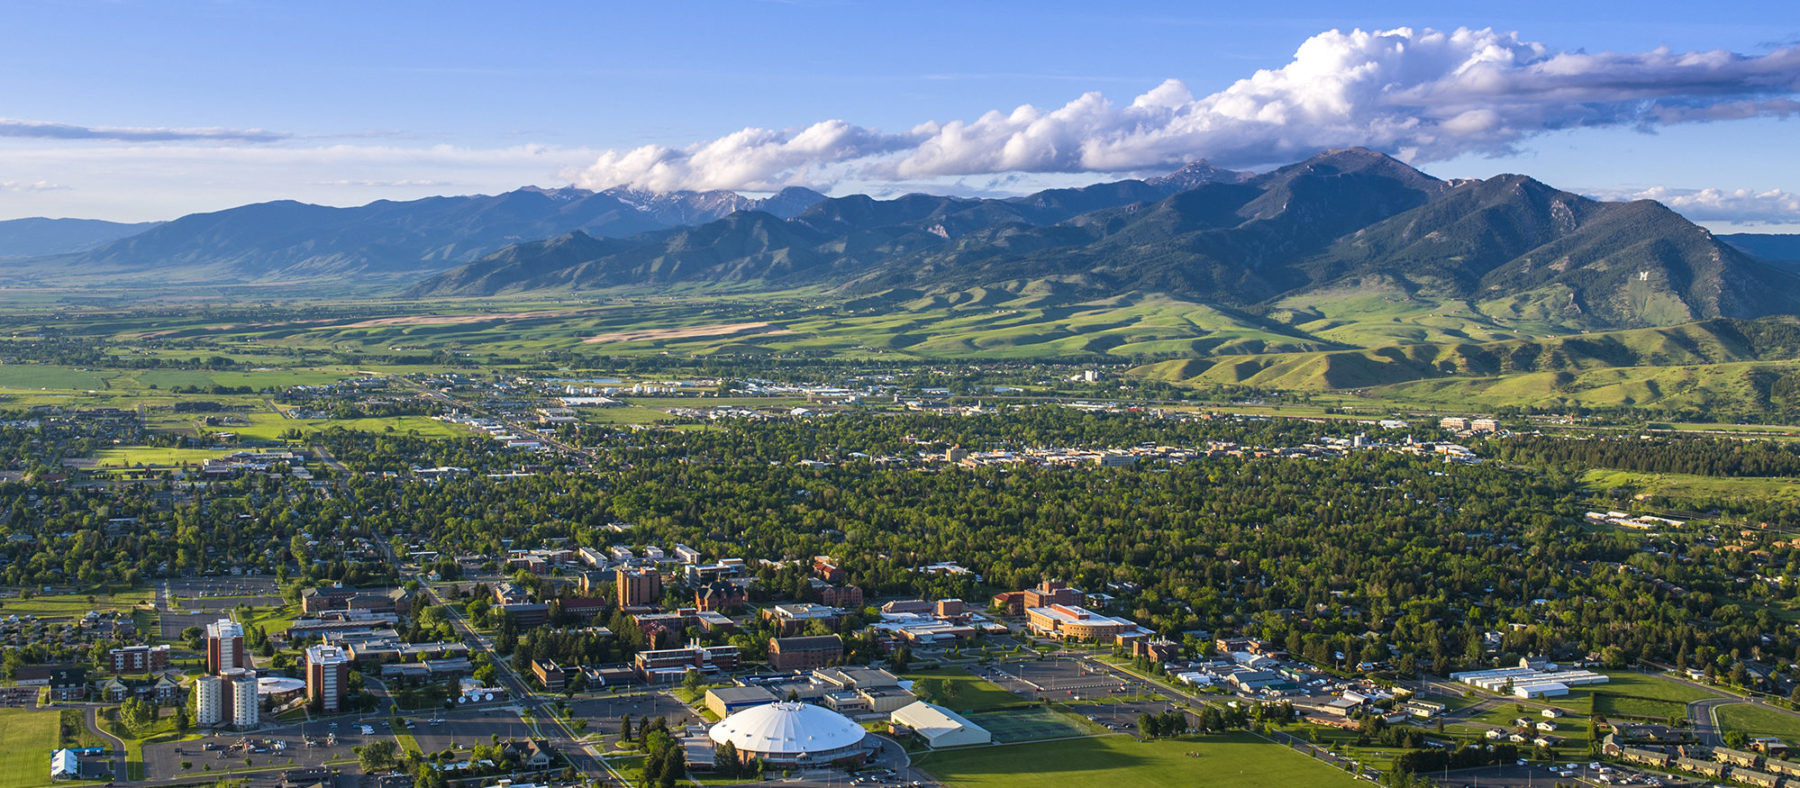
\includegraphics[width=5in,height=\textheight]{images/msu-campus.jpg}}
\usepackage{etoolbox}
\makeatletter
\providecommand{\subtitle}[1]{% add subtitle to \maketitle
  \apptocmd{\@title}{\par {\large #1 \par}}{}{}
}
\makeatother
\subtitle{Spring 2025\\
Montana State University}
\author{Melinda Yager\\
Jade Schmidt\\
Stacey Hancock}
\date{}

\begin{document}
\maketitle

\newpage
\thispagestyle{empty}

This resource was developed by Melinda Yager, Jade Schmidt, and Stacey Hancock in 2021 to accompany the online textbook: Hancock, S., Carnegie, N., Meyer, E., Schmidt, J., and Yager, M. (2021). \emph{Montana State Introductory Statistics with R}. Montana State University. \url{https://mtstateintrostats.github.io/IntroStatTextbook/}.

This resource is released under a \href{https://creativecommons.org/licenses/by-nc-sa/4.0/}{Creative Commons BY-NC-SA 4.0} license unless otherwise noted.

\setcounter{tocdepth}{1}
\addtocontents{toc}{\protect\thispagestyle{empty}}
\tableofcontents
\thispagestyle{empty}

\newpage
\setcounter{page}{1}

\chapter*{Preface}\label{preface}
\addcontentsline{toc}{chapter}{Preface}

This coursepack accompanies the textbook for STAT 216: Montana State Introductory Statistics with R, which can be found at \url{https://mtstateintrostats.github.io/IntroStatTextbook/}. The syllabus for the course (including the course calendar), data sets, and links to D2L Brightspace, Gradescope, and the MSU RStudio server can be found on the course webpage: \url{https://math.montana.edu/courses/s216/}.
Other notes and review materials are linked in D2L.

Each of the activities in this workbook is designed to target specific learning outcomes of the course, giving you practice with important statistical concepts in a group setting with instructor guidance. In addition to the in-class activities for the course, video notes are provided to aid in taking notes while you complete the required videos. Bring this workbook with you to class each class period, and take notes in the workbook as you would your own notes. A well-written completed workbook will provide an optimal study guide for exams!

All activities and labs in this coursepack will be completed during class time. Parts of each lab will be turned in on Gradescope. To aid in your understanding, read through the introduction for each activity before attending class each day.

STAT 216 is a 3-credit in-person course. In our experience, it takes six to nine hours per week outside of class to achieve a good grade in this class. By ``good'' we mean at least a C because a grade of D or below does not count toward fulfilling degree requirements. Many of you set your goals higher than just getting a C, and we fully support that. You need roughly nine hours per week to review past activities, read feedback on previous assignments, complete current assignments, and prepare for the next day's class. A typical week in the life of a STAT 216 student looks like:

\begin{itemize}
\tightlist
\item
  \emph{Prior to class meeting}:

  \begin{itemize}
  \tightlist
  \item
    Read assigned sections of the textbook, using the provided reading guides to take notes on the material.
  \item
    Watch the provided videos, taking notes in the coursepack.
  \item
    Read through the introduction to the day's in-class activity.
  \item
    Read through the week's homework assignment and note any questions you may have on the content.
  \end{itemize}
\item
  \emph{During class meeting}:

  \begin{itemize}
  \tightlist
  \item
    Work through the guided activity, in-class activity or weekly lab with your classmates and instructor, taking detailed notes on your answers to each question in the activity.
  \end{itemize}
\item
  \emph{After class meeting}:

  \begin{itemize}
  \tightlist
  \item
    Complete any parts of the activity you did not complete in class.
  \item
    Review the activity solutions in the Math and Stat Center, and take notes on key points.
  \item
    Complete any remaining assigned readings for the week.
  \item
    Complete the week's homework assignment.
  \end{itemize}
\end{itemize}

\nocite{*}

\chapter{Confidence Intervals for a Single Quantitative Variable}\label{confidence-intervals-for-a-single-quantitative-variable}

\section{Vocabulary Review and Key Topics}\label{vocabulary-review-and-key-topics}

Review the Golden Ticket posted in the resources at the end of the coursepack for a summary of a single quantitative variable.

\subsection{Key topics}\label{key-topics}

Module 7 will cover creating confidence intervals using both simulation-based and theory-based methods. Additionally, we learn about types of errors and power in hypothesis testing.

\subsubsection*{Simulation-based Confidence Interval}\label{simulation-based-confidence-interval}
\addcontentsline{toc}{subsubsection}{Simulation-based Confidence Interval}

\begin{itemize}
\item
  R code to find the simulation-based confidence interval using the \texttt{onemean\_CI} function from the \texttt{catstats} package.

\begin{Shaded}
\begin{Highlighting}[]
\FunctionTok{one\_mean\_CI}\NormalTok{(object}\SpecialCharTok{$}\NormalTok{variable, }\CommentTok{\#Enter the name of the variable}
        \AttributeTok{summary\_measure =} \StringTok{"mean"}\NormalTok{, }\CommentTok{\#choose the mean or median}
        \AttributeTok{number\_repetitions =} \DecValTok{10000}\NormalTok{,  }\CommentTok{\# Number of simulations}
        \AttributeTok{confidence\_level =}\NormalTok{ xx)}
\end{Highlighting}
\end{Shaded}
\item
  Interpretation of the confidence interval is very similar as for a single proportion only the context and summary measure has changed.

  \begin{itemize}
  \item
    To write in context include:

    \begin{itemize}
    \item
      How confident you are (e.g., 90\%, 95\%, 98\%, 99\%)
    \item
      Parameter of interest
    \item
      Calculated interval
    \end{itemize}
  \end{itemize}
\end{itemize}

\subsubsection*{Theory-based Confidence Interval}\label{theory-based-confidence-interval}
\addcontentsline{toc}{subsubsection}{Theory-based Confidence Interval}

\begin{itemize}
\tightlist
\item
  Calculation of the confidence interval for a sample mean:
\end{itemize}

\[\bar{x}\pm t^*\times SE(\bar{x})\]

\begin{itemize}
\item
  R code to find the multiplier for the confidence interval using theory-based methods.

  \begin{itemize}
  \item
    \texttt{qt} will give you the multiplier using the t-distribution with \(n-1\) df (enter for \texttt{yy})
  \item
    Enter the percentile for the given confidence level
  \end{itemize}

\begin{Shaded}
\begin{Highlighting}[]
\FunctionTok{qt}\NormalTok{(percentile, }\AttributeTok{df=}\NormalTok{yy, }\AttributeTok{lower.tail=}\ConstantTok{FALSE}\NormalTok{)}
\end{Highlighting}
\end{Shaded}
\end{itemize}

\newpage

\subsection*{Vocabulary}\label{vocabulary}
\addcontentsline{toc}{subsection}{Vocabulary}

\begin{itemize}
\item
  \textbf{Significance level (\(\alpha\))}: a given cut-off value that we compare the p-value to determine a decision of a test.
\item
  \textbf{Decisions}:

  \begin{itemize}
  \item
    If the p-value is less than the significance level, we make the decision to \emph{reject the null hypothesis}.
  \item
    If the p-value is greater than the significance level, we make the decision to \emph{fail to reject the null hypothesis}.
  \end{itemize}
\item
  \textbf{Type 1 Error}: concluding there is evidence to reject the null hypothesis, when the null is actually true.

  \begin{itemize}
  \tightlist
  \item
    The probability of making a Type 1 error when the null is actually true is equal to the significance level, \(\alpha\).
  \end{itemize}
\item
  \textbf{Type 2 Error}: concluding there is no evidence to reject the null hypothesis, when the null is actually false.
\item
  \textbf{Power}: probability of concluding there is evidence to reject the null hypothesis, when the null is actually false.

  \begin{itemize}
  \tightlist
  \item
    When the null is actually false, the event ``reject the null hypothesis'' is the \emph{complement} of the event ``fail to reject the null hypothesis.'' Thus, power is equal to 1 minus the probability of a Type 2 error.
  \end{itemize}
\end{itemize}

\newpage

\section{Video Notes: Theory-based Inference for a single quantitative variable}\label{video-notes-theory-based-inference-for-a-single-quantitative-variable}

Read Chapters 5 and 17 in the course textbook. Use the following videos to complete the video notes for Module 7.

\subsection{Course Videos}\label{course-videos}

\begin{itemize}
\item
  17.1
\item
  17.3TheoryIntervals
\end{itemize}

\setstretch{1}

\subsection{Single quantitative variable}\label{single-quantitative-variable}

\begin{itemize}
\item
  Reminder: review summary measures and plots discussed in the Module 6 material and Chapter 5 of the textbook.
\item
  The summary measure for a single quantitative variable is the \_\_\_\_\_\_\_\_\_\_\_\_\_\_.
\end{itemize}

\setstretch{1.5}

Notation:

\begin{itemize}
\item
  Population mean:
\item
  Population standard deviation:
\item
  Sample mean:
\item
  Sample standard deviation:
\item
  Sample size:
\end{itemize}

\setstretch{1}

Example: What is the average weight of adult male polar bears? The weight was measured on a representative sample of 83 male polar bears from the Southern Beaufort Sea.

\begin{Shaded}
\begin{Highlighting}[]
\NormalTok{pb }\OtherTok{\textless{}{-}} \FunctionTok{read.csv}\NormalTok{(}\StringTok{"https://math.montana.edu/courses/s216/data/polarbear.csv"}\NormalTok{)}
\end{Highlighting}
\end{Shaded}

Plots of the data:

\begin{Shaded}
\begin{Highlighting}[]
\NormalTok{pb }\SpecialCharTok{\%\textgreater{}\%}
    \FunctionTok{ggplot}\NormalTok{(}\FunctionTok{aes}\NormalTok{(}\AttributeTok{x =}\NormalTok{ Weight)) }\SpecialCharTok{+}   \CommentTok{\# Name variable to plot}
    \FunctionTok{geom\_histogram}\NormalTok{(}\AttributeTok{binwidth =} \DecValTok{10}\NormalTok{) }\SpecialCharTok{+}  \CommentTok{\# Create histogram with specified binwidth}
    \FunctionTok{labs}\NormalTok{(}\AttributeTok{title =} \StringTok{"Histogram of Male Polar Bear Weight"}\NormalTok{, }\CommentTok{\# Title for plot}
       \AttributeTok{x =} \StringTok{"Weight (kg)"}\NormalTok{, }\CommentTok{\# Label for x axis}
       \AttributeTok{y =} \StringTok{"Frequency"}\NormalTok{) }\CommentTok{\# Label for y axis}

\NormalTok{pb }\SpecialCharTok{\%\textgreater{}\%} \CommentTok{\# Data set piped into...}
\FunctionTok{ggplot}\NormalTok{(}\FunctionTok{aes}\NormalTok{(}\AttributeTok{x =}\NormalTok{ Weight)) }\SpecialCharTok{+}   \CommentTok{\# Name variable to plot}
  \FunctionTok{geom\_boxplot}\NormalTok{() }\SpecialCharTok{+}  \CommentTok{\# Create boxplot}
  \FunctionTok{labs}\NormalTok{(}\AttributeTok{title =} \StringTok{"Boxplot of Male Polar Bear Weight"}\NormalTok{, }\CommentTok{\# Title for plot}
       \AttributeTok{x =} \StringTok{"Weight (kg)"}\NormalTok{, }\CommentTok{\# Label for x axis}
       \AttributeTok{y =} \StringTok{"Frequency"}\NormalTok{) }\CommentTok{\# Label for y axis}
\end{Highlighting}
\end{Shaded}

\begin{center}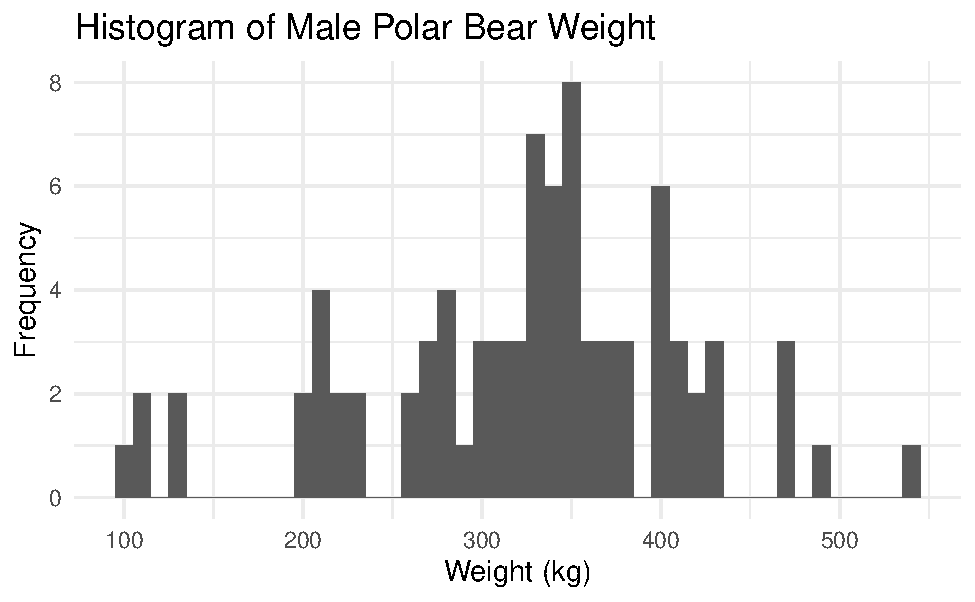
\includegraphics[width=0.6\linewidth]{07-VN07-one_meantheory_files/figure-latex/unnamed-chunk-2-1} 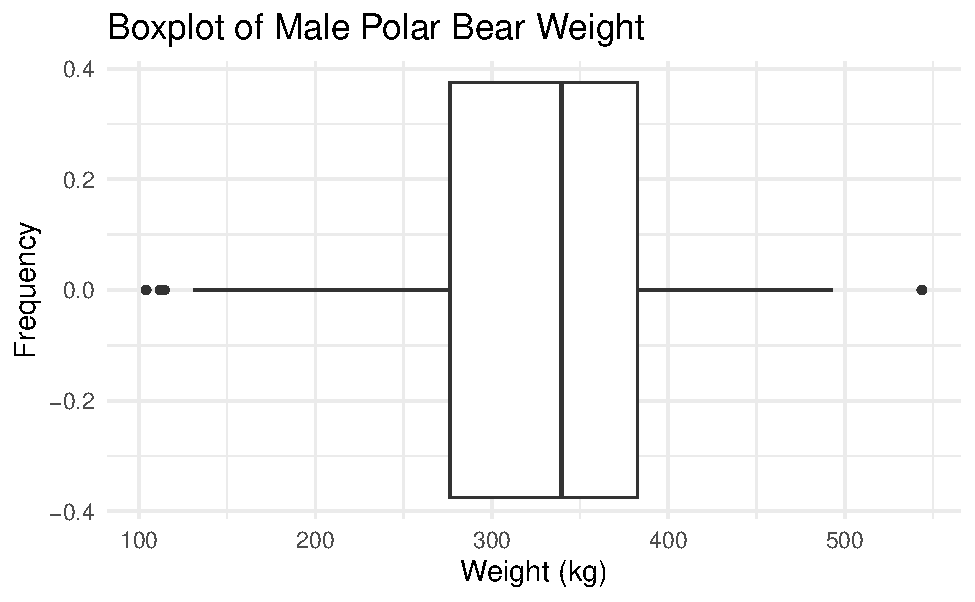
\includegraphics[width=0.6\linewidth]{07-VN07-one_meantheory_files/figure-latex/unnamed-chunk-2-2} \end{center}

Summary Statistics:

\begin{Shaded}
\begin{Highlighting}[]
\NormalTok{pb }\SpecialCharTok{\%\textgreater{}\%}
  \FunctionTok{summarise}\NormalTok{(}\FunctionTok{favstats}\NormalTok{(Weight)) }\CommentTok{\#Gives the summary statistics}
\CommentTok{\#\textgreater{}     min    Q1 median     Q3   max     mean       sd  n missing}
\CommentTok{\#\textgreater{} 1 104.1 276.3  339.4 382.45 543.6 324.5988 88.32615 83       0}
\end{Highlighting}
\end{Shaded}

\subsection*{Confidence interval}\label{confidence-interval}
\addcontentsline{toc}{subsection}{Confidence interval}

\subsubsection*{Simulation-based method}\label{simulation-based-method}
\addcontentsline{toc}{subsubsection}{Simulation-based method}

\begin{itemize}
\item
  Label cards with the values from the data set
\item
  Sample with replacement (bootstrap) from the original sample \(n\) times
\item
  Plot the simulated sample mean on the bootstrap distribution
\item
  Repeat at least 1000 times (simulations)
\item
  Find the cut-offs for the middle X\% (confidence level) in a bootstrap distribution.
\item
  ie. 95\% CI = (2.5th percentile, 97.5th percentile)
\end{itemize}

Conditions for inference for a single mean:

\begin{itemize}
\tightlist
\item
  Independence:
\end{itemize}

\vspace{0.5in}

\begin{Shaded}
\begin{Highlighting}[]
\FunctionTok{set.seed}\NormalTok{(}\DecValTok{216}\NormalTok{)}
\FunctionTok{one\_mean\_CI}\NormalTok{(pb}\SpecialCharTok{$}\NormalTok{Weight,}
  \AttributeTok{summary\_measure =} \StringTok{"mean"}\NormalTok{,}
  \AttributeTok{number\_repetitions =} \DecValTok{10000}\NormalTok{,}
  \AttributeTok{confidence\_level =} \FloatTok{0.95}\NormalTok{)}
\end{Highlighting}
\end{Shaded}

\begin{center}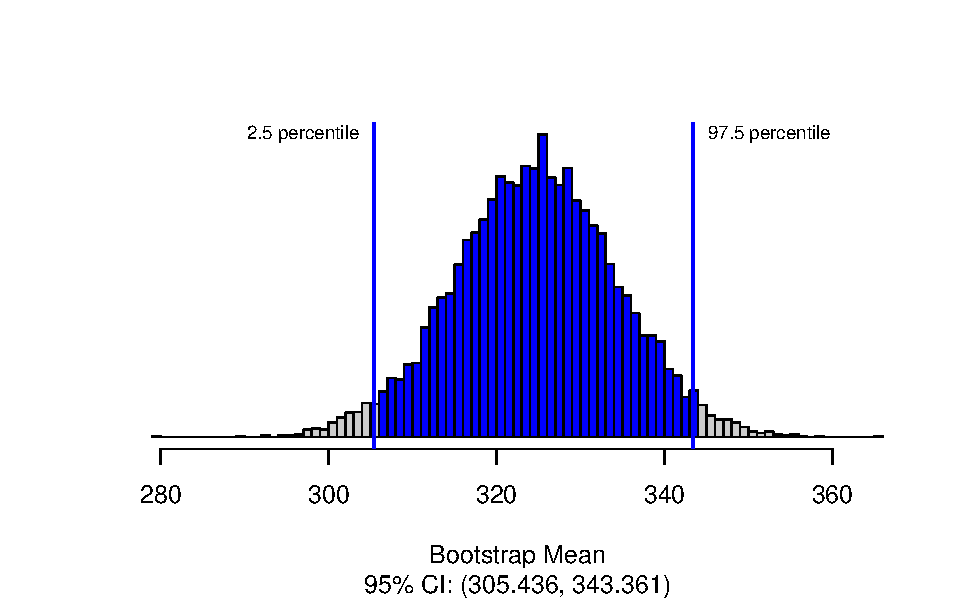
\includegraphics[width=0.7\linewidth]{07-VN07-one_meantheory_files/figure-latex/unnamed-chunk-4-1} \end{center}

The confidence interval estimates the \_\_\_\_\_\_\_\_\_\_\_\_\_\_\_\_
of \_\_\_\_\_\_\_\_\_\_\_\_\_\_\_\_\_\_\_\_.

Confidence interval interpretation:

\begin{itemize}
\item
  How confident you are (e.g., 90\%, 95\%, 98\%, 99\%)
\item
  Parameter of interest
\item
  Calculated interval
\item
  Order of subtraction when comparing two groups
\end{itemize}

\vspace{0.8in}

\newpage

\subsubsection*{Theory-based method}\label{theory-based-method}
\addcontentsline{toc}{subsubsection}{Theory-based method}

\begin{itemize}
\tightlist
\item
  Calculate the interval centered at the sample statistic
\end{itemize}

\rgi \(\text{statistic} \pm \text{margin of error}\)

\vspace{0.5in}

Conditions for inference using theory-based methods:

\begin{itemize}
\tightlist
\item
  Independence:
\end{itemize}

\vspace{0.2in}

\begin{itemize}
\tightlist
\item
  Large enough sample size:
\end{itemize}

\vspace{0.2in}

\subsection*{\texorpdfstring{\(t\)-distribution}{t-distribution}}\label{t-distribution}
\addcontentsline{toc}{subsection}{\(t\)-distribution}

In the theoretical approach, we use the CLT to tell us that the distribution of sample means will be approximately normal, centered at the assumed true mean under \(H_0\) and with standard deviation \(\frac{\sigma}{\sqrt{n}}\).

\[\bar{x} \sim N\left(\mu_0, \frac{\sigma}{\sqrt{n}}\right)\]
\setstretch{1.5}

\begin{itemize}
\item
  Estimate the population standard deviation, \(\sigma\), with the
  \_\_\_\_\_\_\_\_\_\_\_\_\_\_\_\_\_\_\_\_\_\_\_\_\_\_\_ standard deviation, \_\_\_\_\_\_\_\_.
\item
  For a single quantitative variable we use the \_\_\_\_ - distribution
  with \_\_\_\_\_\_\_\_\_\_\_\_\_\_\_
  degrees of freedom to approximate the sampling distribution.
\end{itemize}

\setstretch{1}

The \(t^*\) multiplier is the value at the given percentile of the t-distribution with \(n - 1\) degrees of freedom.

\begin{center}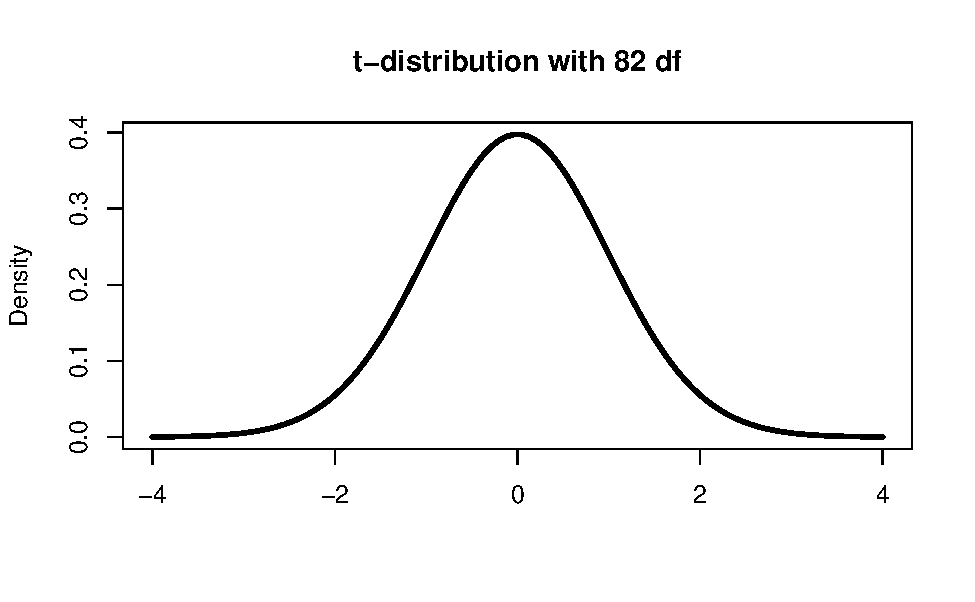
\includegraphics[width=0.7\linewidth]{07-VN07-one_meantheory_files/figure-latex/tstarpb-1} \end{center}

\newpage

To find the \(t^*\) multiplier for a 95\% confidence interval:

\begin{Shaded}
\begin{Highlighting}[]
\FunctionTok{qt}\NormalTok{(}\FloatTok{0.975}\NormalTok{, }\AttributeTok{df =} \DecValTok{82}\NormalTok{)}
\CommentTok{\#\textgreater{} [1] 1.989319}
\end{Highlighting}
\end{Shaded}

Calculation of the confidence interval for the true mean weight of polar bears from the Southern Beaufort Sea:

\vspace{0.8in}

\subsection{Concept Check}\label{concept-check}

Be prepared for group discussion in the next class. One member from the table should write the answers to the following on the whiteboard.

\begin{enumerate}
\def\labelenumi{\arabic{enumi}.}
\tightlist
\item
  Are the conditions met to analyze the polar bear data using theory-based methods?
\end{enumerate}

\vspace{0.7in}

\begin{enumerate}
\def\labelenumi{\arabic{enumi}.}
\setcounter{enumi}{1}
\tightlist
\item
  Interpret the confidence interval found with simulation methods.
\end{enumerate}

\vspace{0.2in}

\newpage

\section{Activity 14: Danceability of Songs}\label{activity-14-danceability-of-songs}

\setstretch{1}

\subsection{Learning outcomes}\label{learning-outcomes}

\begin{itemize}
\item
  Use simulation-based methods to find a confidence interval for a single mean.
\item
  Use theory-based methods to find a confidence interval for a single mean.
\item
  Interpret a confidence interval for a single mean.
\item
  Use a confidence interval to determine the conclusion of a hypothesis test.
\end{itemize}

\subsection{Terminology review}\label{terminology-review}

In today's activity, we will estimate the parameter of interest using simulation-based and theory-based methods. Some terms covered in this activity are:

\begin{itemize}
\item
  Bootstrap distribution
\item
  \(t\)-distribution
\item
  Degrees of freedom
\item
  \(T\)-score
\end{itemize}

To review these concepts, see Chapter 17 in the textbook.

\subsection{Danceability}\label{danceability}

Spotify created a list of the top songs around the world for the past 10 years and several different audio features of those songs. One of the variables measured on these songs is ``danceability.'' Danceability measures how easy it is to dance to a song; the higher the point value the easier it is to dance to the song. Estimate the average danceability of top songs from Spotify.

\begin{itemize}
\item
  Download the R script file for this activity from D2L and upload to the RStudio server.
\item
  Open the R script file, highlight and run the lines to load libraries and the code below.
\end{itemize}

\begin{verbatim}
#>   min Q1 median Q3 max     mean       sd   n missing
#> 1   0 57     66 73  97 64.37977 13.37872 603       0
\end{verbatim}

\begin{Shaded}
\begin{Highlighting}[]
\NormalTok{songs }\SpecialCharTok{\%\textgreater{}\%} \CommentTok{\# Data set piped into...}
    \FunctionTok{ggplot}\NormalTok{(}\FunctionTok{aes}\NormalTok{(}\AttributeTok{x =}\NormalTok{ Danceability)) }\SpecialCharTok{+}   \CommentTok{\# Name variable to plot}
    \FunctionTok{geom\_boxplot}\NormalTok{() }\SpecialCharTok{+}  \CommentTok{\# Create boxplot with specified binwidth}
    \FunctionTok{labs}\NormalTok{(}\AttributeTok{title =} \StringTok{"Boxplot of Danceability Score for Top Spotify Songs"}\NormalTok{, }\CommentTok{\# Title for plot}
         \AttributeTok{x =} \StringTok{"danceability score (points)"}\NormalTok{, }\CommentTok{\# Label for x axis}
         \AttributeTok{y =} \StringTok{""}\NormalTok{) }\SpecialCharTok{+} \CommentTok{\# Remove y axis label}
    \FunctionTok{theme}\NormalTok{(}\AttributeTok{axis.text.y =} \FunctionTok{element\_blank}\NormalTok{(), }
          \AttributeTok{axis.ticks.y =} \FunctionTok{element\_blank}\NormalTok{()) }\CommentTok{\# Removes y{-}axis ticks}
\end{Highlighting}
\end{Shaded}

\begin{center}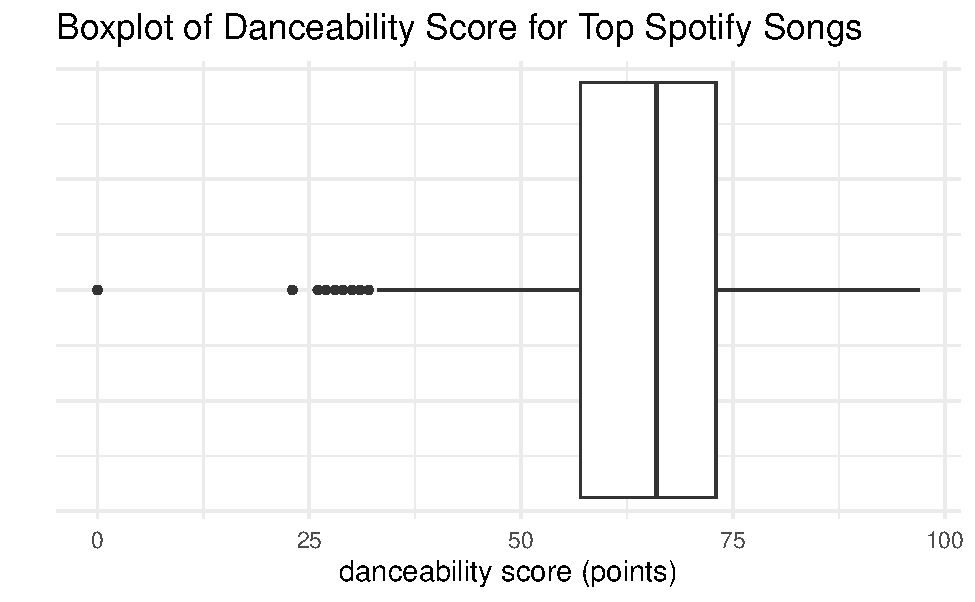
\includegraphics[width=0.7\linewidth]{07-A14-onemean-CI_files/figure-latex/unnamed-chunk-2-1} \end{center}

\subsubsection*{Summarizing quantitative variables}\label{summarizing-quantitative-variables}
\addcontentsline{toc}{subsubsection}{Summarizing quantitative variables}

\begin{enumerate}
\def\labelenumi{\arabic{enumi}.}
\tightlist
\item
  Describe the distribution of danceability of top songs over the past 10 years on Spotify.
\end{enumerate}

\vspace{0.8in}

\begin{enumerate}
\def\labelenumi{\arabic{enumi}.}
\setcounter{enumi}{1}
\tightlist
\item
  Write the parameter of interest in context of the study.
\end{enumerate}

\vspace{0.8in}

\subsection*{Simulation methods to create a confidence interval}\label{simulation-methods-to-create-a-confidence-interval}
\addcontentsline{toc}{subsection}{Simulation methods to create a confidence interval}

Unlike creation of the null distribution, the bootstrap distribution we use for creating a confidence interval is found by sampling with replacement from the original sample. To create one dot on the bootstrap distribution:

\begin{itemize}
\item
  Write the original values for the variable on \(n\) cards; one card for each observational unit.
\item
  Sample with replacement from the cards \(n\) times.
\item
  Plot the mean from each resampled sample on the bootstrap distribution.
\end{itemize}

Use the provided R script file to find a 95\% confidence interval.

\begin{itemize}
\item
  Enter the name of the variable for \texttt{variable}.
\item
  Enter the appropriate confidence level for \texttt{xx}.
\item
  Highlight and run lines 22--25.
\end{itemize}

\begin{Shaded}
\begin{Highlighting}[]
\FunctionTok{one\_mean\_CI}\NormalTok{(songs}\SpecialCharTok{$}\NormalTok{variable, }\CommentTok{\#Enter the name of the variable}
            \AttributeTok{summary\_measure =} \StringTok{"mean"}\NormalTok{, }\CommentTok{\#choose the mean or median}
            \AttributeTok{number\_repetitions =} \DecValTok{10000}\NormalTok{,  }\CommentTok{\# Number of simulations}
            \AttributeTok{confidence\_level =}\NormalTok{ xx)}
\end{Highlighting}
\end{Shaded}

\begin{enumerate}
\def\labelenumi{\arabic{enumi}.}
\setcounter{enumi}{2}
\tightlist
\item
  Report the 95\% confidence interval for the parameter of interest.
\end{enumerate}

\vspace{0.2in}

\subsection*{Theory-based methods to create a confidence interval}\label{theory-based-methods-to-create-a-confidence-interval}
\addcontentsline{toc}{subsection}{Theory-based methods to create a confidence interval}

\begin{itemize}
\item
  \textbf{Conditions for the sampling distribution of \(\bar{x}\) to follow an approximate normal distribution}:

  \begin{itemize}
  \item
    \textbf{Independence}: The sample's observations are independent, e.g., are from a simple random sample. (\emph{Remember}: This also must be true to use simulation methods!)
  \item
    \textbf{Normality Condition}: Either the sample observations come from a normally distributed population or we have a large enough sample size. To check this condition, use the following rules of thumb:

    \begin{itemize}
    \item
      \(n < 30\): The distribution of the sample must be approximately normal with no outliers.
    \item
      \(30 \ge n < 100\): We can relax the condition a little; the distribution of the sample must have no extreme outliers or skewness.
    \item
      \(n > 100\): Can assume the sampling distribution of \(\bar{x}\) is nearly normal, even if the underlying distribution of individual observations is not.
    \end{itemize}
  \end{itemize}
\end{itemize}

Next we will calculate a theory-based confidence interval. To calculate a theory-based confidence interval for the a single mean, use the following formula:

\[\bar{x}\pm t^* \times SE(\bar{x}).\]

We will need to find the \(t^*\) multiplier using the function \texttt{qt()}.

\begin{itemize}
\item
  Enter the appropriate percentile in the R code to find the multiplier for a 95\% confidence interval.
\item
  Enter the degrees of freedom for \texttt{yy}. \emph{The degrees of freedom for a single mean is \(n-1\)}.
\item
  Highlight and run line 31.
\end{itemize}

\begin{Shaded}
\begin{Highlighting}[]
\FunctionTok{qt}\NormalTok{(percentile, }\AttributeTok{df =}\NormalTok{ yy, }\AttributeTok{lower.tail=}\ConstantTok{TRUE}\NormalTok{)}
\end{Highlighting}
\end{Shaded}

\begin{enumerate}
\def\labelenumi{\arabic{enumi}.}
\setcounter{enumi}{3}
\tightlist
\item
  Mark on the \(t\)-distribution found below the values of \(\pm t^*\). Draw a line at each multiplier and write the percentiles used to find each.
  \vspace{1mm}
\end{enumerate}

\begin{figure}

{\centering 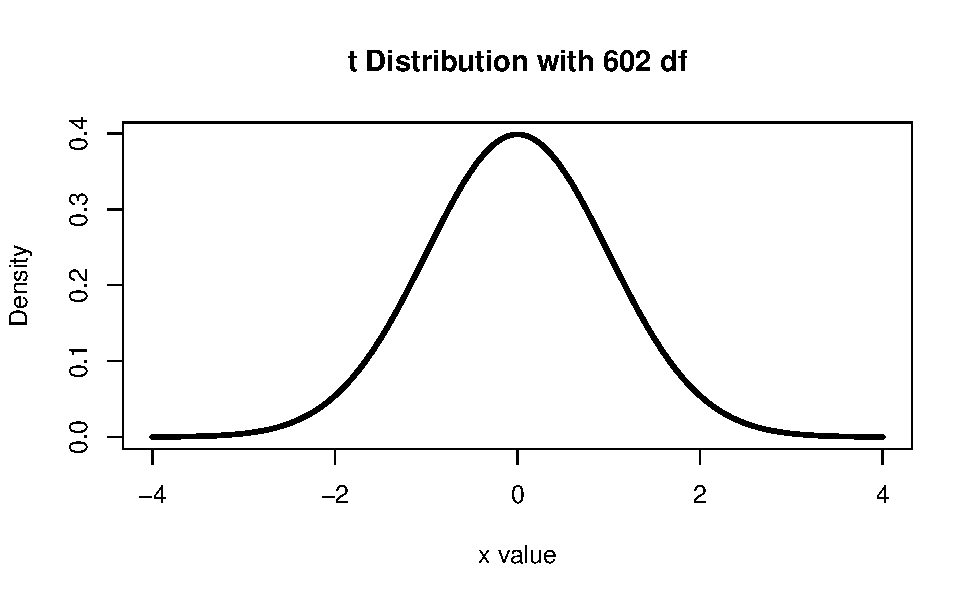
\includegraphics[width=0.75\linewidth]{07-A14-onemean-CI_files/figure-latex/tst-1} 

}

\end{figure}

\newpage

\begin{enumerate}
\def\labelenumi{\arabic{enumi}.}
\setcounter{enumi}{4}
\tightlist
\item
  Calculate the margin of error using theory-based methods.
\end{enumerate}

\vspace{0.6in}

\begin{enumerate}
\def\labelenumi{\arabic{enumi}.}
\setcounter{enumi}{5}
\tightlist
\item
  Calculate the confidence interval for the true mean using theory-based methods.
\end{enumerate}

\vspace{0.6in}

\begin{enumerate}
\def\labelenumi{\arabic{enumi}.}
\setcounter{enumi}{6}
\tightlist
\item
  Interpret the confidence interval in context of the study.
\end{enumerate}

\vspace{1in}

\begin{enumerate}
\def\labelenumi{\arabic{enumi}.}
\setcounter{enumi}{7}
\tightlist
\item
  Explain why the confidence interval with theory-based methods is similar to the confidence interval found using the bootstrap distribution.
\end{enumerate}

\vspace{1in}

\subsection{Take-home messages}\label{take-home-messages}

\begin{enumerate}
\def\labelenumi{\arabic{enumi}.}
\item
  In order to use theory-based methods for a single mean, the independent observational units and normality conditions must be met.
\item
  The simulation-based confidence interval and theory-based confidence interval should be similar if the normality condition is met.
\item
  A \(t^*\) multiplier is found by obtaining the bounds of the middle X\% (X being the desired confidence level) of a \(t\)-distribution with \(n - 1\) df.
\end{enumerate}

\subsection{Additional notes}\label{additional-notes}

Use this space to summarize your thoughts and take additional notes on today's activity and material covered

\newpage

\section{Activity 15: Errors and Power}\label{activity-15-errors-and-power}

\setstretch{1}

\subsection{Learning outcomes}\label{learning-outcomes-1}

\begin{itemize}
\item
  Explain Type I and Type 2 errors in the context of a study.
\item
  Explain the power of a test in the context of a study.
\item
  Understand how changes in sample size, significance level, and the difference between the null value and the parameter value impact the power of a test.
\item
  Understand how significance level impacts the probability of a Type 1 error.
\item
  Understand the relationship between the probability of a Type 2 error and power.
\item
  Be able to distinguish between practical importance and statistical significance.
\end{itemize}

\subsection{Terminology review}\label{terminology-review-1}

In this activity, we will examine the possible errors that can be made based on the decision in a hypothesis test as well as factors influencing the power of the test. Some terms covered in this activity are:

\begin{itemize}
\item
  Significance level
\item
  Type 1 error
\item
  Type 2 error
\item
  Power
\end{itemize}

To review these concepts, see Chapter 12 in the textbook.

\subsection{College textbook cost}\label{college-textbook-cost}

A college student spends, on average, \$280 on textbooks per year. Many universities have started using open-source resources to help defray the cost of textbooks. One such university is hoping to show they have successfully reduced costs by \$100 per year, on average.

\begin{enumerate}
\def\labelenumi{\arabic{enumi}.}
\item
  Write the parameter of interest (\(\mu\)) in words, in the context of this problem.
  \vspace{0.5in}
\item
  Use proper notation to write the null and alternative hypotheses the university would need to test in order to check their claim.
  \vspace{0.5in}
\end{enumerate}

After determining hypotheses and prior to collecting data, researchers should set a \textbf{significance level} for a hypothesis test. The significance level, represented by \(\alpha\) and most commonly 0.01, 0.05, or 0.10, is a cut-off for determining whether a p-value is small or not. The \emph{smaller} the p-value, the \emph{stronger} the evidence against the null hypothesis, so a p-value that is smaller than or equal to the significance level is strong enough evidence to \emph{reject the null hypothesis}. Similarly, the \emph{larger} the p-value, the \emph{weaker} the evidence against the null hypothesis, so a p-value that is larger than the significance level does not provide enough evidence against the null hypothesis and the researcher would \emph{fail to reject the null hypothesis}. Rejecting the null hypothesis or failing to reject the null hypothesis are the two \textbf{decisions} that can be made based on the data collected.

As you have already learned in this course, sample size of a study is extremely important. Often times, researchers will conduct what is called a power analysis to determine the appropriate sample size based on the goals of their research, including a desired \textbf{power} of their test. Power is the probability of correctly rejecting the null hypothesis, or the probability of the data providing strong evidence against the null hypothesis \emph{when the null hypothesis is false}.

The remainder of this activity will be spent investigating how different factors influence the power of a test, after which you will complete a power analysis for this university.

\begin{itemize}
\item
  Navigate to \url{https://istats.shinyapps.io/power/}.
\item
  Choose the tab ``Population Mean''.
\item
  Use the scale under ``Null Hypothesis value \(\mu_0\)'' to change the value to your null value from question 2. *Note we will convert this to a scale in hundreds of dollars (e.g., 1 = \$100). In other words, use the null value of 2.8.
\item
  Change the ``Alternative Hypothesis'' to the direction you wrote in question 2.
\item
  Leave all boxes un-checked.
\item
  Set the ``True value of \(\mu\)'' to 2.8 as well.
\item
  Do not change the scales for ``Sample size n'' or ``Type I Error \(\alpha\)'' or ``Population Std. Dev. \(\sigma\)''.
\end{itemize}

The red distribution you see is the scaled-Normal distribution representing the null distribution for this hypothesis test, if the sample size was \(n = 30\) and the significance level was \(\alpha = 0.05\). This means the red distribution is showing the distribution of possible sample mean amounts spent on textbooks per year (in hundreds of dollars) for a sample of 30 college students (\(\bar{x}\)) if we assume the null hypothesis is true.

\begin{enumerate}
\def\labelenumi{\arabic{enumi}.}
\setcounter{enumi}{2}
\item
  Based off this distribution and your alternative hypothesis, give one possible sample mean which you think would lead to rejecting the null hypothesis. Explain how you decided on your value.
  \vspace{0.25in}
\item
  Check the box for ``Show Critical Value(s) and Rejection Region(s)''. You will now see a vertical line on the plot indicating the \emph{maximum} sample mean which would lead to reject the null hypothesis. That is, any sample means below this value would lead us to reject the null hypothesis; any sample means below this value would lead us to fail to reject the null hypothesis. What is this value?\\
  \vspace{0.25in}
\item
  Notice that there are some sample means under the red line (when the null hypothesis is true) which would lead us to reject the null hypothesis. Give the range of sample means which would lead to rejecting the null hypothesis when the null hypothesis is true? What is the statistical name for this mistake?
  \vspace{0.4in}
\end{enumerate}

Check the ``Type I Error'' box under \textbf{Display}. This should verify (or correct) your answer to question 5! The area shaded in red represents the probability of making a \textbf{Type 1 Error} in our hypothesis test. Recall that a Type 1 error is when we reject the null hypothesis even though the null hypothesis is true. To reject the null hypothesis, the p-value, which was found assuming the null hypothesis is true, must be less than or equal to the significance level. Therefore the significance level is the probability of rejecting the null hypothesis when the null hypothesis is true, so the significance level IS the probability of making a Type 1 error in a hypothesis test!

\begin{enumerate}
\def\labelenumi{\arabic{enumi}.}
\setcounter{enumi}{5}
\tightlist
\item
  Based on the current applet settings, what percent of the null distribution is shaded red (i.e., what is the probability of making a Type 1 error)?
  \vspace{0.25in}
\end{enumerate}

\newpage

Let's say this university believes their program can reduce the cost of textbooks for college students by \$100 per year. In the applet, set the scale under ``True value of \(\mu\)'' to 1.8.

\begin{enumerate}
\def\labelenumi{\arabic{enumi}.}
\setcounter{enumi}{6}
\tightlist
\item
  Where is the blue distribution centered?
  \vspace{0.25in}
\end{enumerate}

The blue distribution that appears represents what the university believes, that \$180 (not \$280) is the true mean textbook cost for college students at this university. This blue distribution represents the idea that the \textbf{null hypothesis is false}.

\begin{enumerate}
\def\labelenumi{\arabic{enumi}.}
\setcounter{enumi}{7}
\tightlist
\item
  Consider the definition of power provided earlier in this activity. Do you believe the power of the test will be an area within the blue distribution or red distribution? How do you know? What about the probability of making a Type 2 error?
  \vspace{1in}
\end{enumerate}

Check the ``Type II Error'' and ``Power'' boxes under \textbf{Display}. This should verify (or correct) your answers to question 8! The area shaded in blue represents the probability of making a \textbf{Type 2 Error} in our hypothesis test (failing to reject the null hypothesis even though the null hypothesis is false). The area shaded in green represents the power of the test. Notice that the Type 1 and Type 2 error rates and the power of the test are provided above the distribution.

\begin{enumerate}
\def\labelenumi{\arabic{enumi}.}
\setcounter{enumi}{8}
\tightlist
\item
  Complete the following equation: Power + Type 2 Error Rate = \_\_\_. Explain why that equation makes sense. \emph{Hint: Consider on what power and Type 2 error are conditional.}
  \vspace{0.6in}
\end{enumerate}

Now let's investigate how changes in different factors influence the power of a test.

\begin{enumerate}
\def\labelenumi{\arabic{enumi}.}
\setcounter{enumi}{9}
\item
  Using the same sample size and significance level, change the ``True value of \(\mu\)'' to see the effect on power.
  \setlength\tabcolsep{0.5cm}

  \begin{longtable}{|l|c|c|c|c|}
  \hline
  \textbf{True value of $p$}& 2.0 & 1.5 & 1.0 & 0.05\\ \hline
  \textbf{Power} & & & &  \\ \hline
  \end{longtable}
\item
  What is changing about the simulated distributions pictured as you change the ``True value of \(\mu\)''?
  \vspace{0.6in}
\item
  How does increasing the distance between the null and believed true mean affect the power of the test?
  \vspace{0.6in}
\end{enumerate}

\newpage

\begin{enumerate}
\def\labelenumi{\arabic{enumi}.}
\setcounter{enumi}{12}
\tightlist
\item
  Using the same significance level, set the ``True value of \(\mu\)'' back to 1.8 and change the sample size to see its effect on power.
\end{enumerate}

\setlength\tabcolsep{0.6cm}
\begin{longtable}{|l|c|c|c|c|c|}
\hline
\textbf{Sample Size}& 20 & 40 & 50 & 60 & 80 \\ \hline
\textbf{Power} & & & & &  \\ \hline
\end{longtable}

\begin{enumerate}
\def\labelenumi{\arabic{enumi}.}
\setcounter{enumi}{13}
\item
  What is changing about the simulated distributions pictured as you change the sample size?
  \vspace{0.6in}
\item
  How does increasing the sample size affect the power of the test?
  \vspace{0.6in}
\item
  Using the same ``True value of \(\mu\)'', set the sample size to 30 and change the ``Type I Error \(\alpha\)'' to see the effect on power.
\end{enumerate}

\setlength\tabcolsep{0.5cm}
\begin{longtable}{|l|c|c|c|c|c|}
\hline
\textbf{Type I Error $\alpha$}& 0.01 & 0.03 & 0.05 & 0.10 & 0.15 \\ \hline
\textbf{Power} & & & & &  \\ \hline
\end{longtable}

\begin{enumerate}
\def\labelenumi{\arabic{enumi}.}
\setcounter{enumi}{16}
\item
  What is changing about the simulated distributions pictured as you change the significance level?
  \vspace{0.6in}
\item
  How does increasing the significance level affect the power of the test?
  \vspace{0.6in}
\item
  Complete the power analysis for this university: The university believes they can reduce the cost of textbooks for their students by \$100. They want to limit the probability of a type 1 error to 10\% and the probability of a type 2 error to 15\%. What is the minimum number of students the university will need to collect data on in order to meet these goals? Use the applet to answer this question.
  \vspace{0.4in}
\item
  Based on the goals outlined in question 19, which mistake below is the university more concerned about? In other words, which of the following two errors were the researchers trying to minimize. Explain your answer.
\end{enumerate}

\begin{itemize}
\item
  Not being able to show their textbook cost is lower, on average, when their textbook cost really is lower.
\item
  Advertising their textbook cost is lower, on average, even though it is not.
\end{itemize}

\vspace{0.8in}

\subsection{Take-home messages}\label{take-home-messages-1}

\begin{enumerate}
\def\labelenumi{\arabic{enumi}.}
\item
  There is a possibility of Type 1 error when we make the decision to reject the null hypothesis. Type 1 error: reject the null hypothesis when the null hypothesis is true. The probability of a Type 1 error when the null hypothesis is true is equal to the significance level, \(\alpha\).
\item
  There is a possibility of Type 2 error when we make the decision to fail to reject the null hypothesis. Type 2 error: fail to reject the null hypothesis when the null hypothesis is false.
\item
  Power of a test is the probability we reject the null when the null hypothesis is false. Power is equal to 1 minus the probability of a Type 2 error.
\item
  Changing the following will \emph{increase} the power of the test:

  \begin{itemize}
  \item
    \emph{Increase} the sample size
  \item
    \emph{Increase} the significance level
  \item
    \emph{Increase} the distance between the null value and the parameter value (note that we don't have control over this!)
  \end{itemize}
\end{enumerate}

\subsection{Additional notes}\label{additional-notes-1}

Use this space to summarize your thoughts and take additional notes on today's activity and material covered.

\newpage

\section{Module 6 and 7 Lab: Arsenic}\label{module-6-and-7-lab-arsenic}

\setstretch{1}

\subsection{Learning outcomes}\label{learning-outcomes-2}

\begin{itemize}
\item
  Given a research question involving one quantitative variable, construct the null and alternative hypotheses
  in words and using appropriate statistical symbols.
\item
  Investigate the process of creating a null distribution for one quantitative variable.
\item
  Find, evaluate, and interpret a p-value from the null distribution.
\item
  Use simulation-based methods to find a confidence interval for a single mean.
\item
  Interpret a confidence interval for a single mean.
\item
  Use a confidence interval to determine the conclusion of a hypothesis test.
\end{itemize}

\subsection{Arsenic}\label{arsenic}

Scientists have devised a new way to measure a person's level of arsenic poisoning by examining toenail clippings. Scientists measured the arsenic levels (in parts per million or ppm) in toenail clippings from 19 randomly selected individuals with private wells in New Hampshire. An arsenic level greater than 0.150 ppm is considered hazardous. Is there evidence the ground water in New Hampshire has hazardous levels of arsenic concentration (as seen in the arsenic levels of New Hampshire residents)? How high is the arsenic concentration for New Hampshire residents with a private well?

\begin{enumerate}
\def\labelenumi{\arabic{enumi}.}
\tightlist
\item
  What does \(\mu\) represent in the context of this study?
\end{enumerate}

\vspace{0.8in}

\begin{enumerate}
\def\labelenumi{\arabic{enumi}.}
\setcounter{enumi}{1}
\tightlist
\item
  Notice that there are two research questions for this study. Identify which research question is best answered by finding a confidence interval and which is best answered by completing a hypothesis test?
\end{enumerate}

\vspace{0.5in}

\begin{enumerate}
\def\labelenumi{\arabic{enumi}.}
\setcounter{enumi}{2}
\tightlist
\item
  Write out the null hypothesis in proper notation for this study.
\end{enumerate}

\vspace{0.4in}

\begin{enumerate}
\def\labelenumi{\arabic{enumi}.}
\setcounter{enumi}{3}
\tightlist
\item
  What sign (\(<\), \(>\), or \(\neq\)) would you use in the alternative hypothesis for this study? Explain your choice.
\end{enumerate}

\vspace{0.5in}

\begin{itemize}
\item
  Upload and open the R script file for Week 12 lab.
\item
  Upload and import the csv file, \texttt{arsenic}.
\item
  Enter the name of the data set (see the environment tab) for \texttt{datasetname} in the R script file in line 11.
\item
  Enter the name of the variable in lines 15
\item
  Write a title for the plot between the quotations and an x-axis label
\item
  Highlight and run lines 1--21 to load the data and create a plot of the data.
\item
  \textbf{Upload a screenshot of your plot to Gradescope}.
\end{itemize}

\begin{Shaded}
\begin{Highlighting}[]
\NormalTok{water }\OtherTok{\textless{}{-}} \FunctionTok{read.csv}\NormalTok{(}\StringTok{"data/arsenic.csv"}\NormalTok{)}
\NormalTok{water }\SpecialCharTok{\%\textgreater{}\%}
    \FunctionTok{summarise}\NormalTok{(}\FunctionTok{favstats}\NormalTok{(variable))}
\NormalTok{water }\SpecialCharTok{\%\textgreater{}\%} \CommentTok{\# Data set piped into...}
    \FunctionTok{ggplot}\NormalTok{(}\FunctionTok{aes}\NormalTok{(}\AttributeTok{x =}\NormalTok{ variable)) }\SpecialCharTok{+}   \CommentTok{\# Name variable to plot}
    \FunctionTok{geom\_boxplot}\NormalTok{() }\SpecialCharTok{+}  \CommentTok{\# Create boxplot with specified binwidth}
    \FunctionTok{labs}\NormalTok{(}\AttributeTok{title =} \StringTok{"Don\textquotesingle{}t forget to title the plot!"}\NormalTok{, }\CommentTok{\# Title for plot}
         \AttributeTok{x =} \StringTok{"Enter an x{-}axis label! Don\textquotesingle{}t forget the units!"}\NormalTok{, }\CommentTok{\# Label for x axis}
         \AttributeTok{y =} \StringTok{""}\NormalTok{) }\SpecialCharTok{+} \CommentTok{\# Remove y axis label}
    \FunctionTok{theme}\NormalTok{(}\AttributeTok{axis.text.y =} \FunctionTok{element\_blank}\NormalTok{(), }
          \AttributeTok{axis.ticks.y =} \FunctionTok{element\_blank}\NormalTok{()) }\CommentTok{\# Removes y{-}axis ticks}
\end{Highlighting}
\end{Shaded}

\begin{enumerate}
\def\labelenumi{\arabic{enumi}.}
\setcounter{enumi}{4}
\item
  Based on the plot, does there appear to be some support in favor of the alternative hypothesis? How do you know?
  \vspace{0.4in}
\item
  Interpret the value of \(Q_3\) in context of the study.
\end{enumerate}

\vspace{0.8in}

\begin{enumerate}
\def\labelenumi{\arabic{enumi}.}
\setcounter{enumi}{6}
\item
  What is the value of \(\bar{x}\)? What is the sample size?
  \vspace{0.25in}
\item
  \textbf{How far, on average, is each arsenic level from the mean arsenic level? What is the appropriate notation for this value?}
\end{enumerate}

\vspace{0.4in}

\subsection*{Use statistical inferential methods to draw inferences from the data}\label{use-statistical-inferential-methods-to-draw-inferences-from-the-data}
\addcontentsline{toc}{subsection}{Use statistical inferential methods to draw inferences from the data}

\begin{enumerate}
\def\labelenumi{\arabic{enumi}.}
\setcounter{enumi}{8}
\tightlist
\item
  Using the provided graphs and summary statistics, determine if both theory-based methods and simulation-based methods could be used to analyze the data. Explain your reasoning.
\end{enumerate}

\vspace{1in}

\subsection*{Hypothesis test}\label{hypothesis-test}
\addcontentsline{toc}{subsection}{Hypothesis test}

Remember that the null distribution is created based on the assumption the null hypothesis is true. In this study, the null hypothesis states that the average arsenic levels are not hazardous.

We will use the \texttt{one\_mean\_test()} function in R (in the \texttt{catstats} package) to simulate the null distribution of sample means and compute a p-value.

\newpage

\begin{enumerate}
\def\labelenumi{\arabic{enumi}.}
\setcounter{enumi}{9}
\tightlist
\item
  Simulate a null distribution and compute the p-value, using the R script file for this lab.
\end{enumerate}

\begin{Shaded}
\begin{Highlighting}[]
\FunctionTok{one\_mean\_test}\NormalTok{(water}\SpecialCharTok{$}\NormalTok{level\_arsenic,   }\CommentTok{\#Enter the name of the variable}
              \AttributeTok{null\_value =} \FloatTok{0.150}\NormalTok{, }\CommentTok{\#Enter the name of the null value}
              \AttributeTok{summary\_measure =} \StringTok{"mean"}\NormalTok{, }\CommentTok{\#Choose mean or median to test}
              \AttributeTok{shift =} \SpecialCharTok{{-}}\FloatTok{0.122}\NormalTok{,  }\CommentTok{\# Shift needed for bootstrap hypothesis test}
              \AttributeTok{as\_extreme\_as =} \FloatTok{0.272}\NormalTok{,  }\CommentTok{\# Observed statistic}
              \AttributeTok{direction =} \StringTok{"greater"}\NormalTok{,  }\CommentTok{\# Direction of alternative}
              \AttributeTok{number\_repetitions =} \DecValTok{10000}\NormalTok{)  }\CommentTok{\# Number of simulated samples for null distribution}
\end{Highlighting}
\end{Shaded}

~~~~~~~Sketch the null distribution created using the \texttt{one\_mean\_test} code.

\vspace{1.5in}

\subsection*{Communicate the results and answer the research question}\label{communicate-the-results-and-answer-the-research-question}
\addcontentsline{toc}{subsection}{Communicate the results and answer the research question}

\begin{enumerate}
\def\labelenumi{\arabic{enumi}.}
\setcounter{enumi}{10}
\tightlist
\item
  \textbf{Report the p-value. Based off of this p-value and a 1\% significance level, what decision would you make about the null hypothesis? What potential error might you be making based on that decision?}
\end{enumerate}

\vspace{0.5in}

\begin{enumerate}
\def\labelenumi{\arabic{enumi}.}
\setcounter{enumi}{11}
\tightlist
\item
  Do you expect the 98\% confidence interval to contain the null value of zero? Explain.
\end{enumerate}

\vspace{0.8in}

\subsection*{Confidence interval}\label{confidence-interval-1}
\addcontentsline{toc}{subsection}{Confidence interval}

We will use the \texttt{one\_mean\_CI()} function in R (in the \texttt{catstats} package) to simulate a bootstrap distribution of sample means and calculate a confidence interval.

\begin{enumerate}
\def\labelenumi{\arabic{enumi}.}
\setcounter{enumi}{12}
\tightlist
\item
  Using bootstrapping and the provided R script file, find a 98\% confidence interval. Fill in the missing values/numbers in the \texttt{one\_mean\_CI()} function to create the 98\% confidence interval.
\end{enumerate}

\begin{Shaded}
\begin{Highlighting}[]
\FunctionTok{one\_mean\_CI}\NormalTok{(}\AttributeTok{data =}\NormalTok{ water}\SpecialCharTok{$}\NormalTok{level\_variable, }\CommentTok{\# Enter vector of differences}
            \AttributeTok{summary\_measure =} \StringTok{"mean"}\NormalTok{,  }\CommentTok{\# Not needed when entering vector of differences}
            \AttributeTok{number\_repetitions =} \DecValTok{10000}\NormalTok{, }\CommentTok{\# Number of bootstrap samples for CI}
            \AttributeTok{confidence\_level =}\NormalTok{ xx)  }\CommentTok{\# Confidence level in decimal form}
\end{Highlighting}
\end{Shaded}

Report the 98\% confidence interval in interval notation.

\vspace{0.3in}

\newpage

\begin{enumerate}
\def\labelenumi{\arabic{enumi}.}
\setcounter{enumi}{13}
\tightlist
\item
  Write a paragraph summarizing the results of the study. \textbf{Upload a copy of your group's paragraph to Gradescope.} Be sure to describe:
\end{enumerate}

\begin{itemize}
\item
  Summary statistic and interpretation

  \begin{itemize}
  \item
    Summary measure (in context)
  \item
    Value of the statistic
  \end{itemize}
\item
  P-value and interpretation

  \begin{itemize}
  \item
    Statement about probability or proportion of samples
  \item
    Statistic (summary measure and value)
  \item
    Direction of the alternative
  \item
    Null hypothesis (in context)
  \end{itemize}
\item
  Confidence interval and interpretation

  \begin{itemize}
  \item
    How confident you are (e.g., 90\%, 95\%, 98\%, 99\%)
  \item
    Parameter of interest
  \item
    Calculated interval
  \end{itemize}
\item
  Conclusion (written to answer the research question)

  \begin{itemize}
  \item
    Amount of evidence
  \item
    Parameter of interest
  \item
    Direction of the alternative hypothesis
  \end{itemize}
\item
  Scope of inference

  \begin{itemize}
  \tightlist
  \item
    To what group of observational units do the results apply (target population or observational units similar to the sample)?
  \end{itemize}
\end{itemize}

\newpage

Paragraph (continued):

\newpage

\phantomsection\label{refs}
\begin{CSLReferences}{1}{0}
\bibitem[\citeproctext]{ref-pga}
{``Average Driving Distance and Fairway Accuracy.''} 2008. \href{https://www.pga.com/\%20and\%20https://www.lpga.com/}{https://www.pga.com/ and https://www.lpga.com/}.

\bibitem[\citeproctext]{ref-banton2022}
Banton, et al, S. 2022. {``Jog with Your Dog: Dog Owner Exercise Routines Predict Dog Exercise Routines and Perception of Ideal Body Weight.''} \emph{PLoS ONE} 17(8).

\bibitem[\citeproctext]{ref-bhavsar2022}
Bhavsar, et al, A. 2022. {``Increased Risk of Herpes Zoster in Adults \(\geq\)50 Years Old Diagnosed with COVID-19 in the United States.''} \emph{Open Forum Infectious Diseases} 9(5).

\bibitem[\citeproctext]{ref-islands}
Bulmer, M. n.d. {``Islands in Schools Project.''} \url{https://sites.google.com/site/islandsinschoolsprojectwebsite/home}.

\bibitem[\citeproctext]{ref-bts}
{``Bureau of Transportation Statistics.''} 2019. \url{https://www.bts.gov/}.

\bibitem[\citeproctext]{ref-babies}
{``Child Health and Development Studies.''} n.d. \url{https://www.chdstudies.org/}.

\bibitem[\citeproctext]{ref-darley1973}
Darley, J. M., and C. D. Batson. 1973. {``"From Jerusalem to Jericho": A Study of Situational and Dispositional Variables in Helping Behavior.''} \emph{Journal of Personality and Social Psychology} 27: 100--108.

\bibitem[\citeproctext]{ref-davis2020}
Davis, Smith, A. K. 2020. {``A Poor Substitute for the Real Thing: Captive-Reared Monarch Butterflies Are Weaker, Paler and Have Less Elongated Wings Than Wild Migrants.''} \emph{Biology Letters} 16.

\bibitem[\citeproctext]{ref-doit2015}
Du Toit, et al, G. 2015. {``Randomized Trial of Peanut Consumption in Infants at Risk for Peanut Allergy.''} \emph{New England Journal of Medicine} 372.

\bibitem[\citeproctext]{ref-edmunds2016}
Edmunds, et al, D. 2016. {``Chronic Wasting Disease Drives Population Decline of White-Tailed Deer.''} \emph{PLoS ONE} 11(8).

\bibitem[\citeproctext]{ref-ipeds}
Education Statistics, National Center for. 2018. {``IPEDS.''} \url{https://nces.ed.gov/ipeds/}.

\bibitem[\citeproctext]{ref-gbmarried}
{``Great Britain Married Couples: Great Britain Office of Population Census and Surveys.''} n.d. \url{https://discovery.nationalarchives.gov.uk/details/r/C13351}.

\bibitem[\citeproctext]{ref-zeitler2012}
Group, TODAY Study. 2012. {``\href{https://www.ncbi.nlm.nih.gov/pubmed/22540912}{A Clinical Trial to Maintain Glycemic Control in Youth with Type 2 Diabetes}.''} \emph{New England Journal of Medicine} 366: 2247--56.

\bibitem[\citeproctext]{ref-hamblin2007}
Hamblin, J. K., K. Wynn, and P. Bloom. 2007. {``Social Evaluation by Preverbal Infants.''} \emph{Nature} 450 (6288): 557--59.

\bibitem[\citeproctext]{ref-hirschfelder2018}
Hirschfelder, A., and P. F. Molin. 2018. {``I Is for Ignoble: Stereotyping Native Americans.''} \href{Retrieved\%20from\%20https://www.ferris.edu/HTMLS/news/jimcrow/native/homepage.htm.}{Retrieved from https://www.ferris.edu/HTMLS/news/jimcrow/native/homepage.htm.}

\bibitem[\citeproctext]{ref-hutchison2013}
Hutchison, R. L., and M. A. Hirthler. 2013. {``\href{https://www.ncbi.nlm.nih.gov/pubmed/23932117}{Upper Extremity Injuies in Homer's Iliad}.''} \emph{Journal of Hand Surgery (American Volume)} 38: 1790--93.

\bibitem[\citeproctext]{ref-imdb}
{``{IMDb} Movies Extensive Dataset.''} 2016. \url{https://kaggle.com/stefanoleone992/imdb-extensive-dataset}.

\bibitem[\citeproctext]{ref-kalra2022}
Kalra, et al., Dl. 2022. {``Trustworthiness of Indian Youtubers.''} Kaggle. \url{https://doi.org/10.34740/KAGGLE/DSV/4426566}.

\bibitem[\citeproctext]{ref-keating2021}
Keating, D., N. Ahmed, F. Nirappil, Stanley-Becker I., and L. Bernstein. 2021. {``Coronavirus Infections Dropping Where People Are Vaccinated, Rising Where They Are Not, Post Analysis Finds.''} \emph{Washington Post}. \url{https://www.washingtonpost.com/health/2021/06/14/covid-cases-vaccination-rates/}.

\bibitem[\citeproctext]{ref-laeng2007}
Laeng, Mathisen, B. 2007. {``Why Do Blue-Eyed Men Prefer Women with the Same Eye Color?''} \emph{Behavioral Ecology and Sociobiology} 61(3).

\bibitem[\citeproctext]{ref-levin2000}
Levin, D. T. 2000. {``Race as a Visual Feature: Using Visual Search and Perceptual Discrimination Tasks to Understand Face Categories and the Cross-Race Recognition Deficit.''} \emph{Journal of Experimental Psychology} 129(4).

\bibitem[\citeproctext]{ref-luetkemeier2017}
LUETKEMEIER, et al., M. 2017. {``Skin Tattoos Alter Sweat Rate and Na+ Concentration.''} \emph{Medicine and Science in Sports and Exercise} 49(7).

\bibitem[\citeproctext]{ref-madden2020}
Madden, et al, J. 2020. {``Ready Student One: Exploring the Predictors of Student Learning in Virtual Reality.''} \emph{PLoS ONE} 15(3).

\bibitem[\citeproctext]{ref-miller1956}
Miller, G. A. 1956. {``The Magical Number Seven, Plus or Minus Two: Some Limits on Our Capacity for Processing Information.''} \emph{Psychological Review} 63(2).

\bibitem[\citeproctext]{ref-becentispeech}
Moquin, W., and C. Van Doren. 1973. {``Great Documents in American Indian History.''} Praeger.

\bibitem[\citeproctext]{ref-pew2022}
{``More Americans Are Joining the 'Cashless' Economy.''} 2022. \url{https://www.pewresearch.org/short-reads/2022/10/05/more-americans-are-joining-the-cashless-economy/.}

\bibitem[\citeproctext]{ref-weather}
National Weather Service Corporate Image Web Team. n.d. {``National Weather Service -- {NWS} Billings.''} \url{https://w2.weather.gov/climate/xmacis.php?wfo=byz}.

\bibitem[\citeproctext]{ref-obrien2019}
O'Brien, Lynch, H. D. 2019. {``Crocodylian Head Width Allometry and Phylogenetic Prediction of Body Size in Extinct Crocodyliforms.''} \emph{Integrative Organismal Biology} 1.

\bibitem[\citeproctext]{ref-ocean}
{``Ocean Temperature and Salinity Study.''} n.d. \url{https://calcofi.org/}.

\bibitem[\citeproctext]{ref-WashPost2022}
{``Older People Who Get Covid Are at Increased Risk of Getting Shingles.''} 2022. \url{https://www.washingtonpost.com/health/2022/04/19/shingles-and-covid-over-50/.}

\bibitem[\citeproctext]{ref-physhealth}
{``Physician's Health Study.''} n.d. \url{https://phs.bwh.harvard.edu/}.

\bibitem[\citeproctext]{ref-porath2017}
Porath, Erez, C. 2017. {``Does Rudeness Really Matter? The Effects of Rudeness on Task Performance and Helpfulness.''} \emph{Academy of Management Journal} 50.

\bibitem[\citeproctext]{ref-quinn1999}
Quinn, G. E., C. H. Shin, M. G. Maguire, and R. A. Stone. 1999. {``Myopia and Ambient Lighting at Night.''} \emph{Nature} 399 (6732): 113--14. \url{https://doi.org/10.1038/20094}.

\bibitem[\citeproctext]{ref-ramachandran2007}
Ramachandran, V. 2007. {``3 Clues to Understanding Your Brain.''} \url{https://www.ted.com/talks/vs_ramachandran_3_clues_to_understanding_your_brain}.

\bibitem[\citeproctext]{ref-cdchospitalization}
{``Rates of Laboratory-Confimed COVID-19 Hospitalizations by Vaccination Status.''} 2021. CDC. \url{https://covid.cdc.gov/covid-data-tracker/\#covidnet-hospitalizations-vaccination}.

\bibitem[\citeproctext]{ref-richardson2019}
Richardson, T., and R. T. Gilman. 2019. {``Left-Handedness Is Associated with Greater Fighting Success in Humans.''} \emph{Scientific Reports} 9 (1): 15402. \url{https://doi.org/10.1038/s41598-019-51975-3}.

\bibitem[\citeproctext]{ref-stephens2020}
Stephens, R., and O. Robertson. 2020. {``Swearing as a Response to Pain: Assessing Hypoalgesic Effects of Novel "Swear" Words.''} \emph{Frontiers in Psychology} 11: 643--62.

\bibitem[\citeproctext]{ref-stewart2014}
Stewart, E. H., B. Davis, B. L. Clemans-Taylor, B. Littenberg, C. A. Estrada, and R. M. Centor. 2014. {``Rapid Antigen Group a Streptococcus Test to Diagnose Pharyngitis: A Systematic Review and Meta-Analysis''} 9 (11). \url{https://doi.org/10.1371/journal.pone.0111727}.

\bibitem[\citeproctext]{ref-stroop1935}
Stroop, J. R. 1935. {``Studies of Interference in Serial Verbal Reactions.''} \emph{Journal of Experimental Psychology} 18: 643--62.

\bibitem[\citeproctext]{ref-subach2022}
Subach, et al, A. 2022. {``Foraging Behaviour, Habitat Use and Population Size of the Desert Horned Viper in the Negev Desert.''} \emph{Soc.Open Sci} 9.

\bibitem[\citeproctext]{ref-sulheim2017}
Sulheim, S., A. Ekeland, I. Holme, and R. Bahr. 2017. {``Helmet Use and Risk of Head Injuries in Alpine Skiers and Snowboarders: Changes After an Interval of One Decade''} 51 (1): 44--50. \url{https://doi.org/10.1136/bjsports-2015-095798}.

\bibitem[\citeproctext]{ref-titanic}
{``Titanic.''} n.d. \url{http://www.encyclopedia-titanica.org}.

\bibitem[\citeproctext]{ref-covidvaccinetracker}
{``US COVID-19 Vaccine Tracker: See Your State's Progress.''} 2021. Mayo Clinic. \url{https://www.mayoclinic.org/coronavirus-covid-19/vaccine-tracker}.

\bibitem[\citeproctext]{ref-usepa2020}
US Environmental Protection Agency. n.d. {``Air Data -- Daily Air Quality Tracker.''} \url{https://www.epa.gov/outdoor-air-quality-data/air-data-daily-air-quality-tracker}.

\bibitem[\citeproctext]{ref-wahlstrom2014}
Wahlstrom, et al, K. 2014. {``Examining the Impact of Later School Start Times on the Health and Academic Performance of High School Students: A Multi-Site Study.''} \emph{Center for Applied Research and Educational Improvement}.

\bibitem[\citeproctext]{ref-watson2015}
Watson, et al., N. 2015. {``Recommended Amount of Sleep for a Heathy Adult: A Joint Consensus Statement of the American Academy of Sleep Medicine and Sleep Research Society.''} \emph{Sleep} 38(6).

\bibitem[\citeproctext]{ref-Weiss1988}
Weiss, R. D. 1988. {``Relapse to Cocaine Abuse After Initiating Desipramine Treatment.''} \emph{JAMA} 260(17).

\bibitem[\citeproctext]{ref-navajo2011}
{``Welcome to the Navajo Nation Government: Official Site of the Navajo Nation.''} 2011.\href{\%20Retrieved\%20from\%20https://www.navajo-nsn.gov/.}{Retrieved from https://www.navajo-nsn.gov/.}

\bibitem[\citeproctext]{ref-wilson2016}
Wilson, Woodruff, J. P. 2016. {``Vertebral Adaptations to Large Body Size in Theropod Dinosaurs.''} \emph{PLoS ONE} 11(7).

\end{CSLReferences}

\end{document}
